\section{Water}

\begin{multicols}{2}


\section*{Occurrence and Nature \hfill \\ of Water}


\subsection{The Water Cycle}

\begin{center}
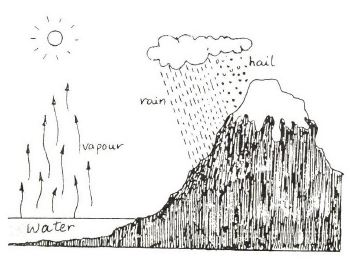
\includegraphics[width=0.4\textwidth]{./img/source/water-cycle.jpg}
\end{center}

\begin{description*}
%\item[Subtopic:]{}
\item[Materials:]{Cards, scissors}
%\item[Setup:]{}
\item[Procedure:]{Cut out cards and label them according to different terms associated with the water cycle (e.g. evaporation, condensation, precipitation, transpiration, collection). Sketch the picture shown and have students label where each takes place.}
%\item[Hazards:]{}
%\item[Questions:]{}
%\item[Observations:]{}
%\item[Theory:]{}
%\item[Applications:]{}
%\item[Notes:]{}
\end{description*}

\subsection{Cloud in a Jar}

%\begin{center}
%\includegraphics[width=0.4\textwidth]{./img/.jpg}
%\end{center}

\begin{description*}
%\item[Subtopic:]{}
\item[Materials:]{Wide mouth glass jar, balloon/latex glove, water, matches}
%\item[Setup:]{}
\item[Procedure:]{Add a small amount of water to the jar. Stretch the mouth of the balloon around the mouth of the jar and insert it so it hangs in the bottle. Pull the balloon out and quickly open the seal and drop in a lit match. Quickly reseal, pushing the balloon back inside the bottle, and then pull the balloon outside of the jar again.}
%\item[Hazards:]{}
%\item[Questions:]{}
\item[Observations:]{A cloud forms inside the jar.}
\item[Theory:]{By putting the balloon in the jar and pulling it out, the volume inside the container increases and some of the water turns into vapour. Dropping a match creates smoke and other particles where rain can form. Pulling the balloon out again lowers the temperature by decreasing the volume enough to start forming clouds.}
\item[Applications:]{Clouds in the sky are formed when water vapour is cooled to form tiny water droplets.}
%\item[Notes:]{}
\end{description*}

%==================================================================================================%

\section*{Properties of Water}


\subsection{Test for Water} % LASM 76 PIC!!!

%\begin{center}
%\includegraphics[width=0.4\textwidth]{./img/.jpg}
%\end{center}

\begin{description*}
%\item[Subtopic:]{}
\item[Materials:]{Copper (II) sulphate, spoon, candle, water}
%\item[Setup:]{}
\item[Procedure:]{Place a small amount of blue copper (II) sulphate in a metal spoon. Heat the spoon over the candle until the crystals have changed from blue to white. Add a few drops of water to the white crystals. }
%\item[Hazards:]{}
%\item[Questions:]{}
%\item[Observations:]{}
\item[Theory:]{On heating blue hydrated copper (II) sulphate, the colour changes from blue
($\mathrm{Cu}\mathrm{SO}_4\cdot 5\mathrm{H}_2\mathrm{O}$) to white ($\mathrm{Cu}\mathrm{SO}_4$). On addition of a few drops of water $\mathrm{Cu}\mathrm{SO}_4$ returns to its original hydrated state (blue), i.e. copper sulphate pentahydrated.}
%\item[Applications:]{}
%\item[Notes:]{}
\end{description*}

%==================================================================================================%

\section*{Importance of Water}


\subsection{Wasted Water}

\begin{center}
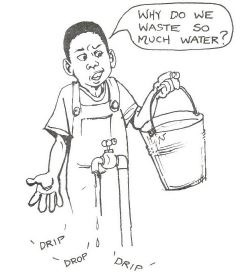
\includegraphics[width=0.4\textwidth]{./img/source/water-waste.jpg}
\end{center}

\begin{description*}
%\item[Subtopic:]{}
%\item[Materials:]{}
%\item[Setup:]{}
\item[Procedure:]{Conduct an experiment or survey at your school or village. If you have a dripping tap or leaking pipe, try to find out how much water it wastes each day. Collect the water and measure the volume lost over 15 minutes and then calculate how much would be lost in a day, week, etc.}
%\item[Hazards:]{}
%\item[Questions:]{}
%\item[Observations:]{}
%\item[Theory:]{}
\item[Applications:]{Water is essential for all life. Many areas have very little access to water. What can you do in your community to reduce water waste?}
%\item[Notes:]{}
\end{description*}

\columnbreak

\subsection{Water in Daily Life}

\begin{center}
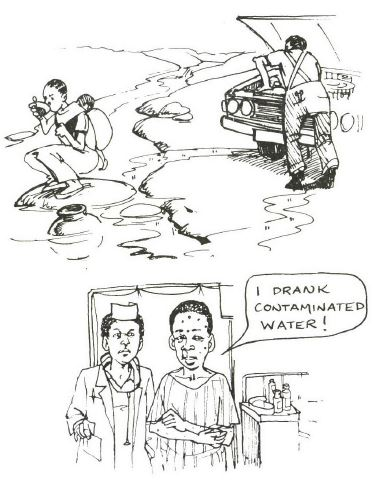
\includegraphics[width=0.4\textwidth]{./img/source/water-daily-life.jpg}
\end{center}

\begin{description*}
%\item[Subtopic:]{}
%\item[Materials:]{}
%\item[Setup:]{}
\item[Procedure:]{Ask the students to
talk about:

(a) The importance of water in daily life;

(b) Where and why water is being polluted;

(c) How contaminated water may harm people.}
%\item[Hazards:]{}
%\item[Questions:]{}
%\item[Observations:]{}
\item[Theory:]{(b) People washing or urinating in/near
rivers, lakes; used lubricating oil of cars etc.
being dumped on soil may enter the ground
water table; factories using chemicals (e.g.
tanneries, paper mills, fertilizer plants, pesticide
plants etc.) may pollute rivers, lakes etc.

(c) People may get typhoid fever, cholera etc.
when drinking contaminated water from rivers,
lakes or wells; water contaminated by factories
may cause cancer etc.}
%\item[Applications:]{}
%\item[Notes:]{}
\end{description*}

%==================================================================================================%

\section*{Treatment and Purification of Water}


\subsection{The `SODIS' Method} % PIC!!!

%\begin{center}
%\includegraphics[width=0.4\textwidth]{./img/.jpg}
%\end{center}

\begin{description*}
%\item[Subtopic:]{}
%\item[Materials:]{}
%\item[Setup:]{}
\item[Procedure:]{Fill a bottle with water from a tap. Place it on the roof of your house in open sunlight for 2 days or 3-4 days if it is cloudy. Filter through a clean cloth or kanga.}
%\item[Hazards:]{}
%\item[Questions:]{}
%\item[Observations:]{}
\item[Theory:]{Ultraviolet rays from the sun kill the harmful bacteria in the water that cause disease. Filtering though a cloth removes solid impurities.}
%\item[Applications:]{}
%\item[Notes:]{}
\end{description*}

\columnbreak

\subsection{Constructing a Water Filter}

\begin{center}
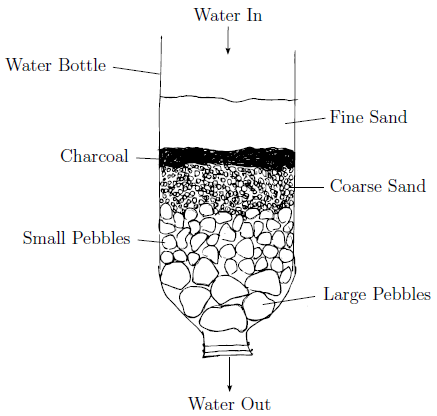
\includegraphics[width=0.4\textwidth]{./img/water-filter.png}
\end{center}

\begin{description*}
%\item[Subtopic:]{}
\item[Materials:]{Fine sand, coarse sand, small pebbles, large pebbles, charcoal, empty bottle, dirty water}
\item[Setup:]{Rinse off all pebbles and remove and dirt from the sand. Cut the bottom of a bottle so it is shaped like a funnel.}
\item[Procedure:]{Invert the bottle and place the large pebbles, followed by smaller pebbles, coarse sand, charcoal and sand on top. Run water through until it comes out clean on bottom.}
%\item[Hazards:]{}
%\item[Questions:]{}
%\item[Observations:]{}
\item[Theory:]{When dirty water passes through sand particles, impurities are trapped and
remain above. The smallest particles and some micro-organisms are stopped
by the charcoal layer.}
%\item[Applications:]{}
%\item[Notes:]{}
\end{description*}

%\vfill
%\columnbreak

\subsection{Water Treatment at Home}

%\begin{center}
%\includegraphics[width=0.4\textwidth]{./img/.jpg}
%\end{center}

\begin{description*}
%\item[Subtopic:]{}
\item[Materials:]{\nameref{sec:heatsources}, pot, water, clean cloth, bucket}
%\item[Setup:]{}
\item[Procedure:]{Boil a pot of water and let it cool. Then pour through a clean cloth or kanga into a clean bucket. The water is now safe for drinking.}
%\item[Hazards:]{}
%\item[Questions:]{}
%\item[Observations:]{}
\item[Theory:]{Boiling water at the boiling point (100$^\circ$C) kills the germs and
bacteria which may cause diseases. Filtration with a piece of clean white
cloth removes any solid impurities.}
%\item[Applications:]{}
%\item[Notes:]{}
\end{description*}

%==================================================================================================%


\end{multicols}

\pagebreak